\documentclass[a4paper, 12pt]{article}

\usepackage{hyperref}
\usepackage[warn]{mathtext}
\usepackage[utf8]{inputenc}
\usepackage[T2A]{fontenc}
\usepackage[english,russian]{babel}
\usepackage{multirow}
\usepackage{amsmath,amsfonts,amssymb,amsthm,mathtools}
\usepackage{indentfirst}
\DeclareSymbolFont{T2Aletters}{T2A}{cmr}{m}{it}
\usepackage{ gensymb }
\mathtoolsset{showonlyrefs=true}
\usepackage{euscript}
\usepackage{mathrsfs}
\usepackage[left=2cm,right=2cm,top=2cm,bottom=2cm]{geometry}
\usepackage{graphicx}
\usepackage{wrapfig}
\usepackage[rgb]{xcolor}
\hypersetup{
colorlinks=true,
urlcolor=blue
}


\title{Лабораторная работа}
\author{Гисич Арсений Б03-102}
\date{2022}

\begin{document}

	\begin{center}
		{\large МОСКОВСКИЙ ФИЗИКО-ТЕХНИЧЕСКИЙ ИНСТИТУТ (НАЦИОНАЛЬНЫЙ ИССЛЕДОВАТЕЛЬСКИЙ УНИВЕРСИТЕТ)}
	\end{center}
	\vspace{5 cm}
	{\Large
		\begin{center}
			{\bf Лабораторная работа 3.2.1}\\[0.2 cm]
			Сдвиг фаз в цепи переменного тока
		\end{center}
	}
	\vspace{4 cm}
	\begin{flushright}
		{\Large Выполнил: \\
			\vspace{0.2 cm}
			Гисич Арсений \\
			\vspace{0.2 cm}
			Б03-102 \\}
	\end{flushright}
	\vspace{9 cm}
	\begin{center}
		Долгопрудный\\[0.1 cm]
		2022
	\end{center}
\thispagestyle{empty}

\section{Аннотация}

В данной работе были исследованы вынужденные колебания в цепи переменного тока, вызываемые меняющейся по гармоническому закону ЭДС. Измерен сдвиг фаз между вызывающей колебания ЭДС и колебаниями тока в цепи, а также зависимость величины сдвига от активного сопротивления в цепи.

\section{Теоретические сведения}

\begin{wrapfigure}{r}{0.3\textwidth}
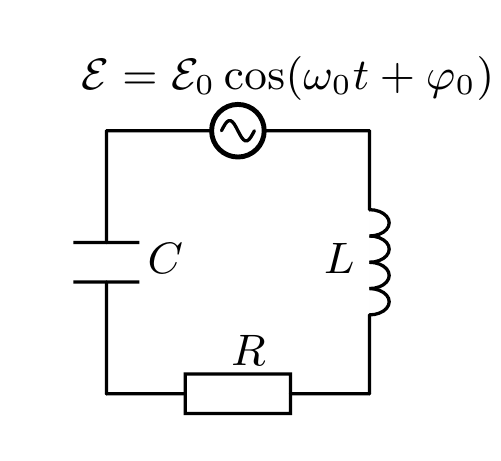
\includegraphics[width=0.3\textwidth]{1.png}
\caption{Последовательный контур с внешней ЭДС}
\label{r1}
\end{wrapfigure}

Рассмотрим процессы, протекающие в контуре, подключённом к источнику внешней ЭДС, изменяющейся по гармоническому закону $\varepsilon = \varepsilon_0 \cos{(\omega t + \varphi_0)}$. Для напряжения на конденсаторе $U_C(t)$ получим уравнение 
\begin{equation}\label{eq1}
\ddot{U}_C + 2\gamma \dot{U}_C + \omega_0^2U_С = \varepsilon_0\cos{(\omega t + \varphi_0)}.
\end{equation}

Перейдём к комплексному представлению колебаний. Запишем уравнение~\eqref{eq1} в комплексной форме, обозначая комплексные величины как <<векторы>>:
\begin{align}\label{eq2}
U_C & = \mathrm{Re}\,\mathbf{U_C}, & \mathbf{U_C} & = \mathrm{Re}\,\mathbf{U_C} + i\,\mathrm{Im}\,\mathbf{U_C}, \\
\varepsilon & = \mathrm{Re}\,\mathbf{\varepsilon}, & \mathbf{\varepsilon} & = \mathbf{\varepsilon_0}e^{i\omega t} = \varepsilon_0e^{i(\omega t + \varphi_0)},
\end{align}
\begin{equation}\label{eq3}
\mathbf{\ddot{U}_C} + 2\gamma \mathbf{\dot{U}_C} + \omega_0^2\mathbf{U_С} = \omega_0^2\mathbf{\varepsilon}.
\end{equation}

Комплексный множитель $\mathbf{\varepsilon_0} = \varepsilon_0e^{i\varphi_0}$, стоящий перед $e^{i\omega t}$, называется \textit{комплексной амплитудой}.

Решив уравнение~\eqref{eq3}, получим комплескное выражение для напряжения на конденсаторе $\mathbf{U_C}$. \textit{Вещественная часть} этого решения $\mathrm{Re}\,\mathbf{U_C}$ и является решением исходного уравнения~\eqref{eq1}. Будем искать решение уравнения~\eqref{eq3} в виде
\begin{equation}\label{eq4}
\mathbf{U_C}(t) = \mathbf{U_{C0}}e^{i\omega t},
\end{equation}
где $\mathbf{U_{C0}}$ --- комплексная амплитуда напряжения на конденсаторе, не зависящая от времени. Подставляя \eqref{eq4} в \eqref{eq3}, находим $\mathbf{U_{C0}}$ и далее, комплексные амплитуды тока в контуре и напряжений на сопротивлении и индуктивности:
\begin{equation}\label{eq5}
\mathbf{U_{C0}} = \frac{\mathbf{\varepsilon_0}}{i\omega CZ}, \quad Z = R + i\left(\omega L - \frac{1}{\omega C}\right),
\end{equation}
\begin{equation}\label{eq6}
\mathbf{I_0} = \frac{\mathbf{\varepsilon_0}}{Z}, \quad \mathbf{U_{R0}} = \frac{R\mathbf{\varepsilon_0}}{Z}, \quad \mathbf{U_{L0}} = i\omega L\frac{\mathbf{\varepsilon_0}}{Z}.
\end{equation}

Комплексная величина $Z$ называется \textit{комплексным сопротивлением}, или \textit{импедансом}, последовательного контура. Можно определить импеданс каждого отдельного элемента контура:
\begin{equation}\label{eq7}
Z_R = R, \quad Z_L = i\omega L, \quad Z_C = \frac{1}{i\omega C}.
\end{equation}

В новых обозначениях уравнения \eqref{eq5}--\eqref{eq6} принимают вид
\begin{equation}\label{eq8}
\mathbf{I} = \frac{\mathbf{\varepsilon_0}}{Z}, \quad \mathbf{U_{R0}} = Z_R\mathbf{I_0}, \quad \mathbf{U_{C0}} = Z_C\mathbf{I_0}, \quad \mathbf{U_{L0}} = Z_L\mathbf{I_0}.
\end{equation}

Импеданс контура $Z$ не зависит от начальных условий, не содержит величин ни токов, ни напряжений, а определяется свойствами всех элементов, соединённых в контур, и частотой синусоидальной ЭДС, к которой он подключён. Таким образом, \textit{импеданс $Z$ является характеристикой колебательного контура на заданной частоте}.

Выражение \eqref{eq5} для импеданса контура $Z$ содержит действительную часть $$\mathrm{Re}\,Z = R,$$ называемую \textit{активным} сопротивлением контура, и мнимую часть $$\mathrm{Im}\,Z = \omega L - \frac{1}{\omega C},$$ носящую название \textit{реактивного} сопротивления.

Импедансы контура и его отдельных элементов --- комплексные числа --- могут быть представленны в показательной форме:
\begin{equation}\label{eq9}
Z = Z_0e^{i\psi},
\end{equation}
где $Z_0 = |Z|$ --- модуль комплексного числа, $\psi = \arg{Z}$ --- его аргумент (фаза). Для импеданса рассматриваемого последовательного контура при этом находим
\begin{equation}\label{eq10}
Z_0 = \sqrt{(\mathrm{Re}\,Z)^2 + (\mathrm{Im}\,Z)^2} = \sqrt{R^2 + \left(\omega L - \frac{1}{\omega C}\right)^2} = \frac{R}{\cos{\psi_I}},
\end{equation}
\begin{equation}\label{eq11}
\tan{\psi_I} = \frac{\mathrm{Im}\,Z}{\mathrm{Re}\,Z} = \frac{\omega L - \frac{1}{\omega C}}{R}.
\end{equation}
Ток в контуре и напряжения на отдельных его элементах теперь могут быть получены по формулам~\eqref{eq5}--\eqref{eq8}. Например, действительная часть тока в контуре
\begin{equation}\label{eq12}
I(t) = \frac{\varepsilon_0}{R}\cos{\psi_I}\cos({\omega t + \varphi_0 - \psi_I)}.
\end{equation}
Как видно из~\eqref{eq11}~и~\eqref{eq12}, угол~$\psi_I$, определяемый отношением мнимой и действительной частей импеданса, представляют собой сдвиг фаз между напряжением на последовательном контуре и током в нём, причём \textit{положительные значения угла~$\psi_I$ соответствуют отставанию фазы тока, а отрицательные --- опережению}. В общем случае, когда к источнику последовательно подключены резистор, конденсатор и катушка самоиндукции, сдвиг фазы $\psi_I$ лежит в пределах $-\pi/2 < \psi_I < \pi/2$.

\section{Методика измерений}

Схема установки для исследования сдвига фаз между током и напряжением в цепи переменного тока представленна на рис.~\ref{r2}. Эталонная катушка $L$, магазин ёмкостей $C$ и магазин сопротивлений $R$ соединены последовательно и через дополнительное сопротивление $r$ подключены к источнику синусоидального напряжения --- звуковому генератору.

\begin{figure}[h!]
\begin{flushleft}
    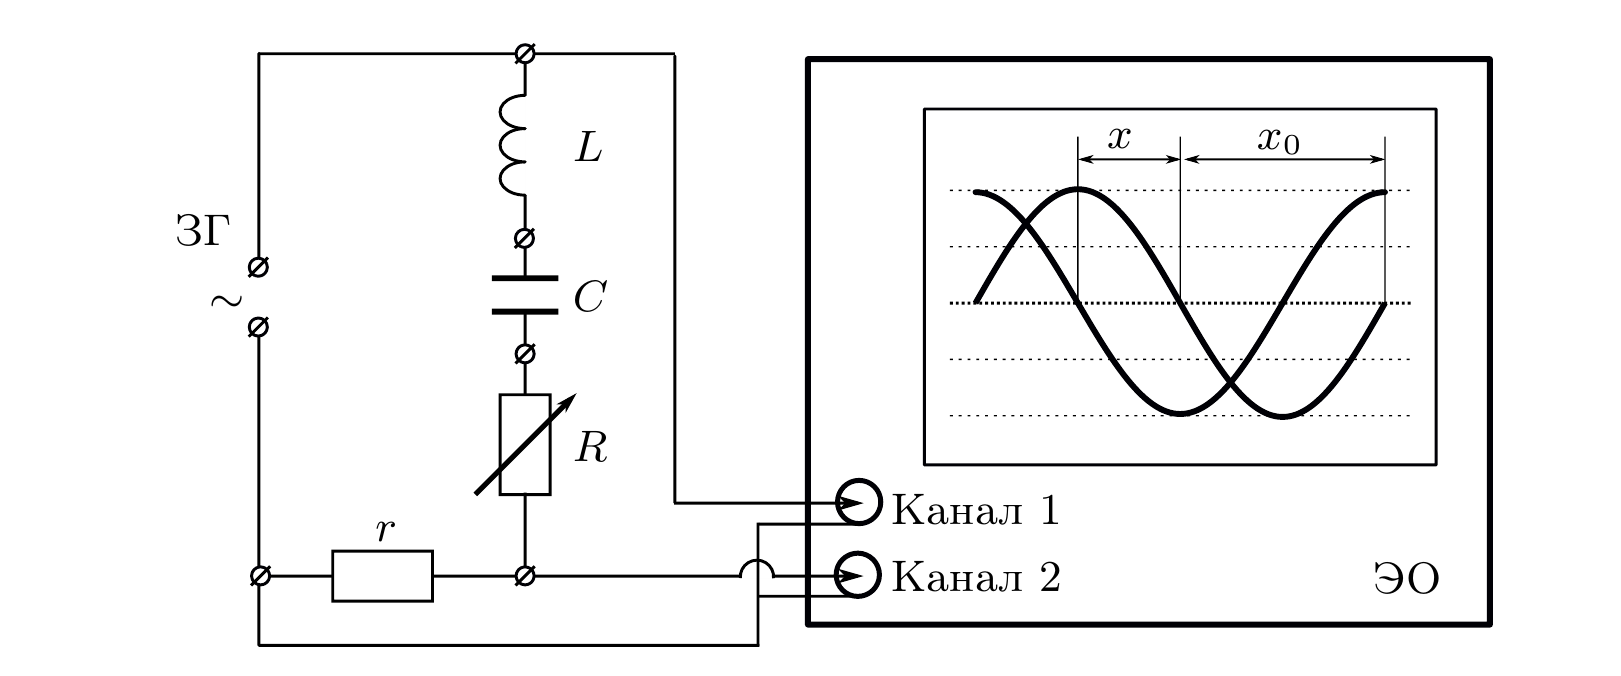
\includegraphics[scale=2.3]{2.png}
\end{flushleft}
\caption{Схема установки для исследования сдвига фаз между током и напряжением}
\label{r2}
\end{figure}

Сигнал, пропорциональный току, снимается с сопротивления $r$, пропорциональный напряжению, --- с генератора. Оба сигнала подаются на осциллограф, имеющий два канала вертикального отклонения.

На практике часто используют устройства, называемые \textit{фазовращателями}, которые позволяют изменять фазу напряжения в широких пределах ($0 < \psi < \pi$). Схема фазовращателя, применяемого в данной работе, изображена на рис.~\ref{r3}. Она содержит два одинаковых резистора $R_1$, смонтированных на отдельной плате, магазин сопротивлений $R$ и магазин ёмкостей $C$.

\begin{figure}[h!]
\begin{flushleft}
    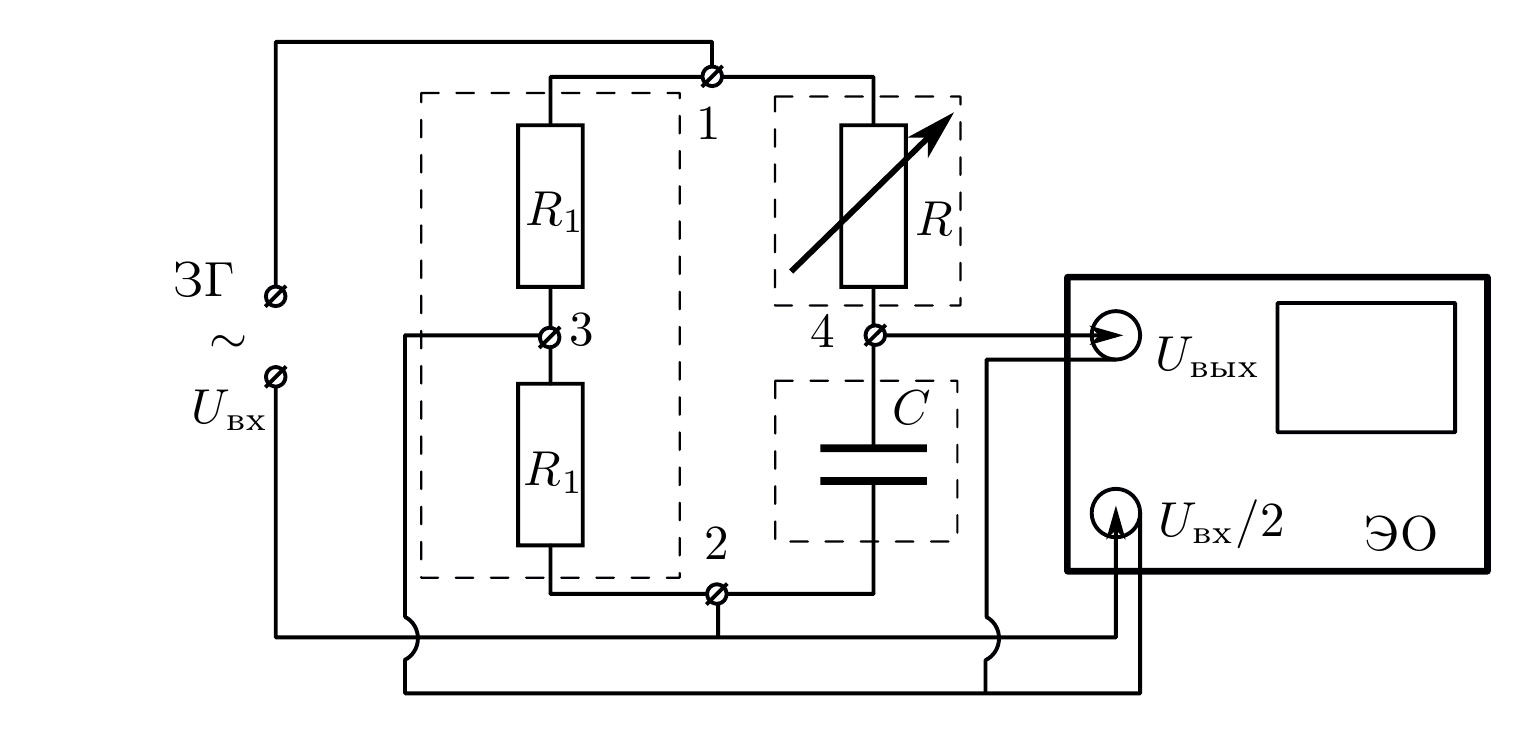
\includegraphics[scale=2.2]{3.png}
\end{flushleft}
\caption{Схема установки для исследования фазовращателя}
\label{r3}
\end{figure}

Сдвиг фаз между выходным и входным напряжениями равен
\begin{equation}
\psi = \arg{\frac{U_{вых}}{U_{вх}}} = 2\arctg{\frac{1}{\omega RC}}.
\end{equation}
Он может меняться от $\psi = \pi$ при $R \rightarrow 0$ до $\psi = 0$ при $R \rightarrow \infty$.

\section{Используемое оборудование}

\begin{enumerate}
    \item генератор звуковой частоты;
    \item двухканальный осциллограф;
    \item магазин ёмкостей;
    \item магазин сопротивлений;
    \item катушка индуктивности;
    \item резисторы;
    \item универсальный измеритель импеданса ($LCR$-метр);
\end{enumerate}

\section{Результаты измерений и обработка данных}

\subsection{RC-цепь}

Установленные параметры: $C = 0,5~мкФ,\; \nu = 1~кГц$. Рассчитанное реактивное сопротивление цепи $X_1 = 1/(\omega C) = 318~Ом$. Полученные значения сдвига фаз $\psi$ в зависимости от сопротивления $R$ представленны в таблице \ref{tab1}.

\begin{table}[h!]
\begin{center}
\begin{tabular}{|c|c|c|c|c|c|c|c|}
\hline
$R, Ом$   & $\sigma_R, Ом$ & $x_0, дел$ & $\sigma_{x_0}, дел$ & $x, дел$ & $\sigma_x, дел$ & $\psi, \pi \cdot рад$ & $\sigma_{\psi}, \pi \cdot рад$ \\ \hline
0,00    & 0,01   & 25,0    & 0,5      & -12,0  & 0,5     & -0,48       & 0,02        \\ \hline
300,00  & 0,01   & 25,0    & 0,5      & -6,5   & 0,5     & -0,26       & 0,02        \\ \hline
600,00  & 0,01   & 25,0    & 0,5      & -4,0   & 0,5     & -0,16       & 0,02        \\ \hline
900,00  & 0,01   & 25,0    & 0,5      & -2,5   & 0,5     & -0,10       & 0,02        \\ \hline
1800,00 & 0,01   & 25,0    & 0,5      & -1,0   & 0,5     & -0,04       & 0,02        \\ \hline
320,00  & 0,01   & 25,0    & 0,5      & -6,0   & 0,5     & -0,24       & 0,02        \\ \hline
240,00  & 0,01   & 25,0    & 0,5      & -7,0   & 0,5     & -0,28       & 0,02        \\ \hline
190,00  & 0,01   & 25,0    & 0,5      & -8,0   & 0,5     & -0,32       & 0,02        \\ \hline
\end{tabular}
\end{center}
\caption{RC-цепь}
\label{tab1}
\end{table}

Полученный график зависимости $ctg\,\psi = f(\omega CR_{\Sigma})$ представлен на рис.~\ref{ris1}. Синим цветом нарисована экспериментальная зависимость, оранжевым --- теоретическая --- \\ $ctg\,\psi = - \omega CR_{\Sigma}$. Погрешность экспериментально полученного коэффициента зависимости составляет $\sigma_{RC} = 39~\%$, что является существенной погрешностью.

\begin{figure}[h!]
\begin{flushleft}
    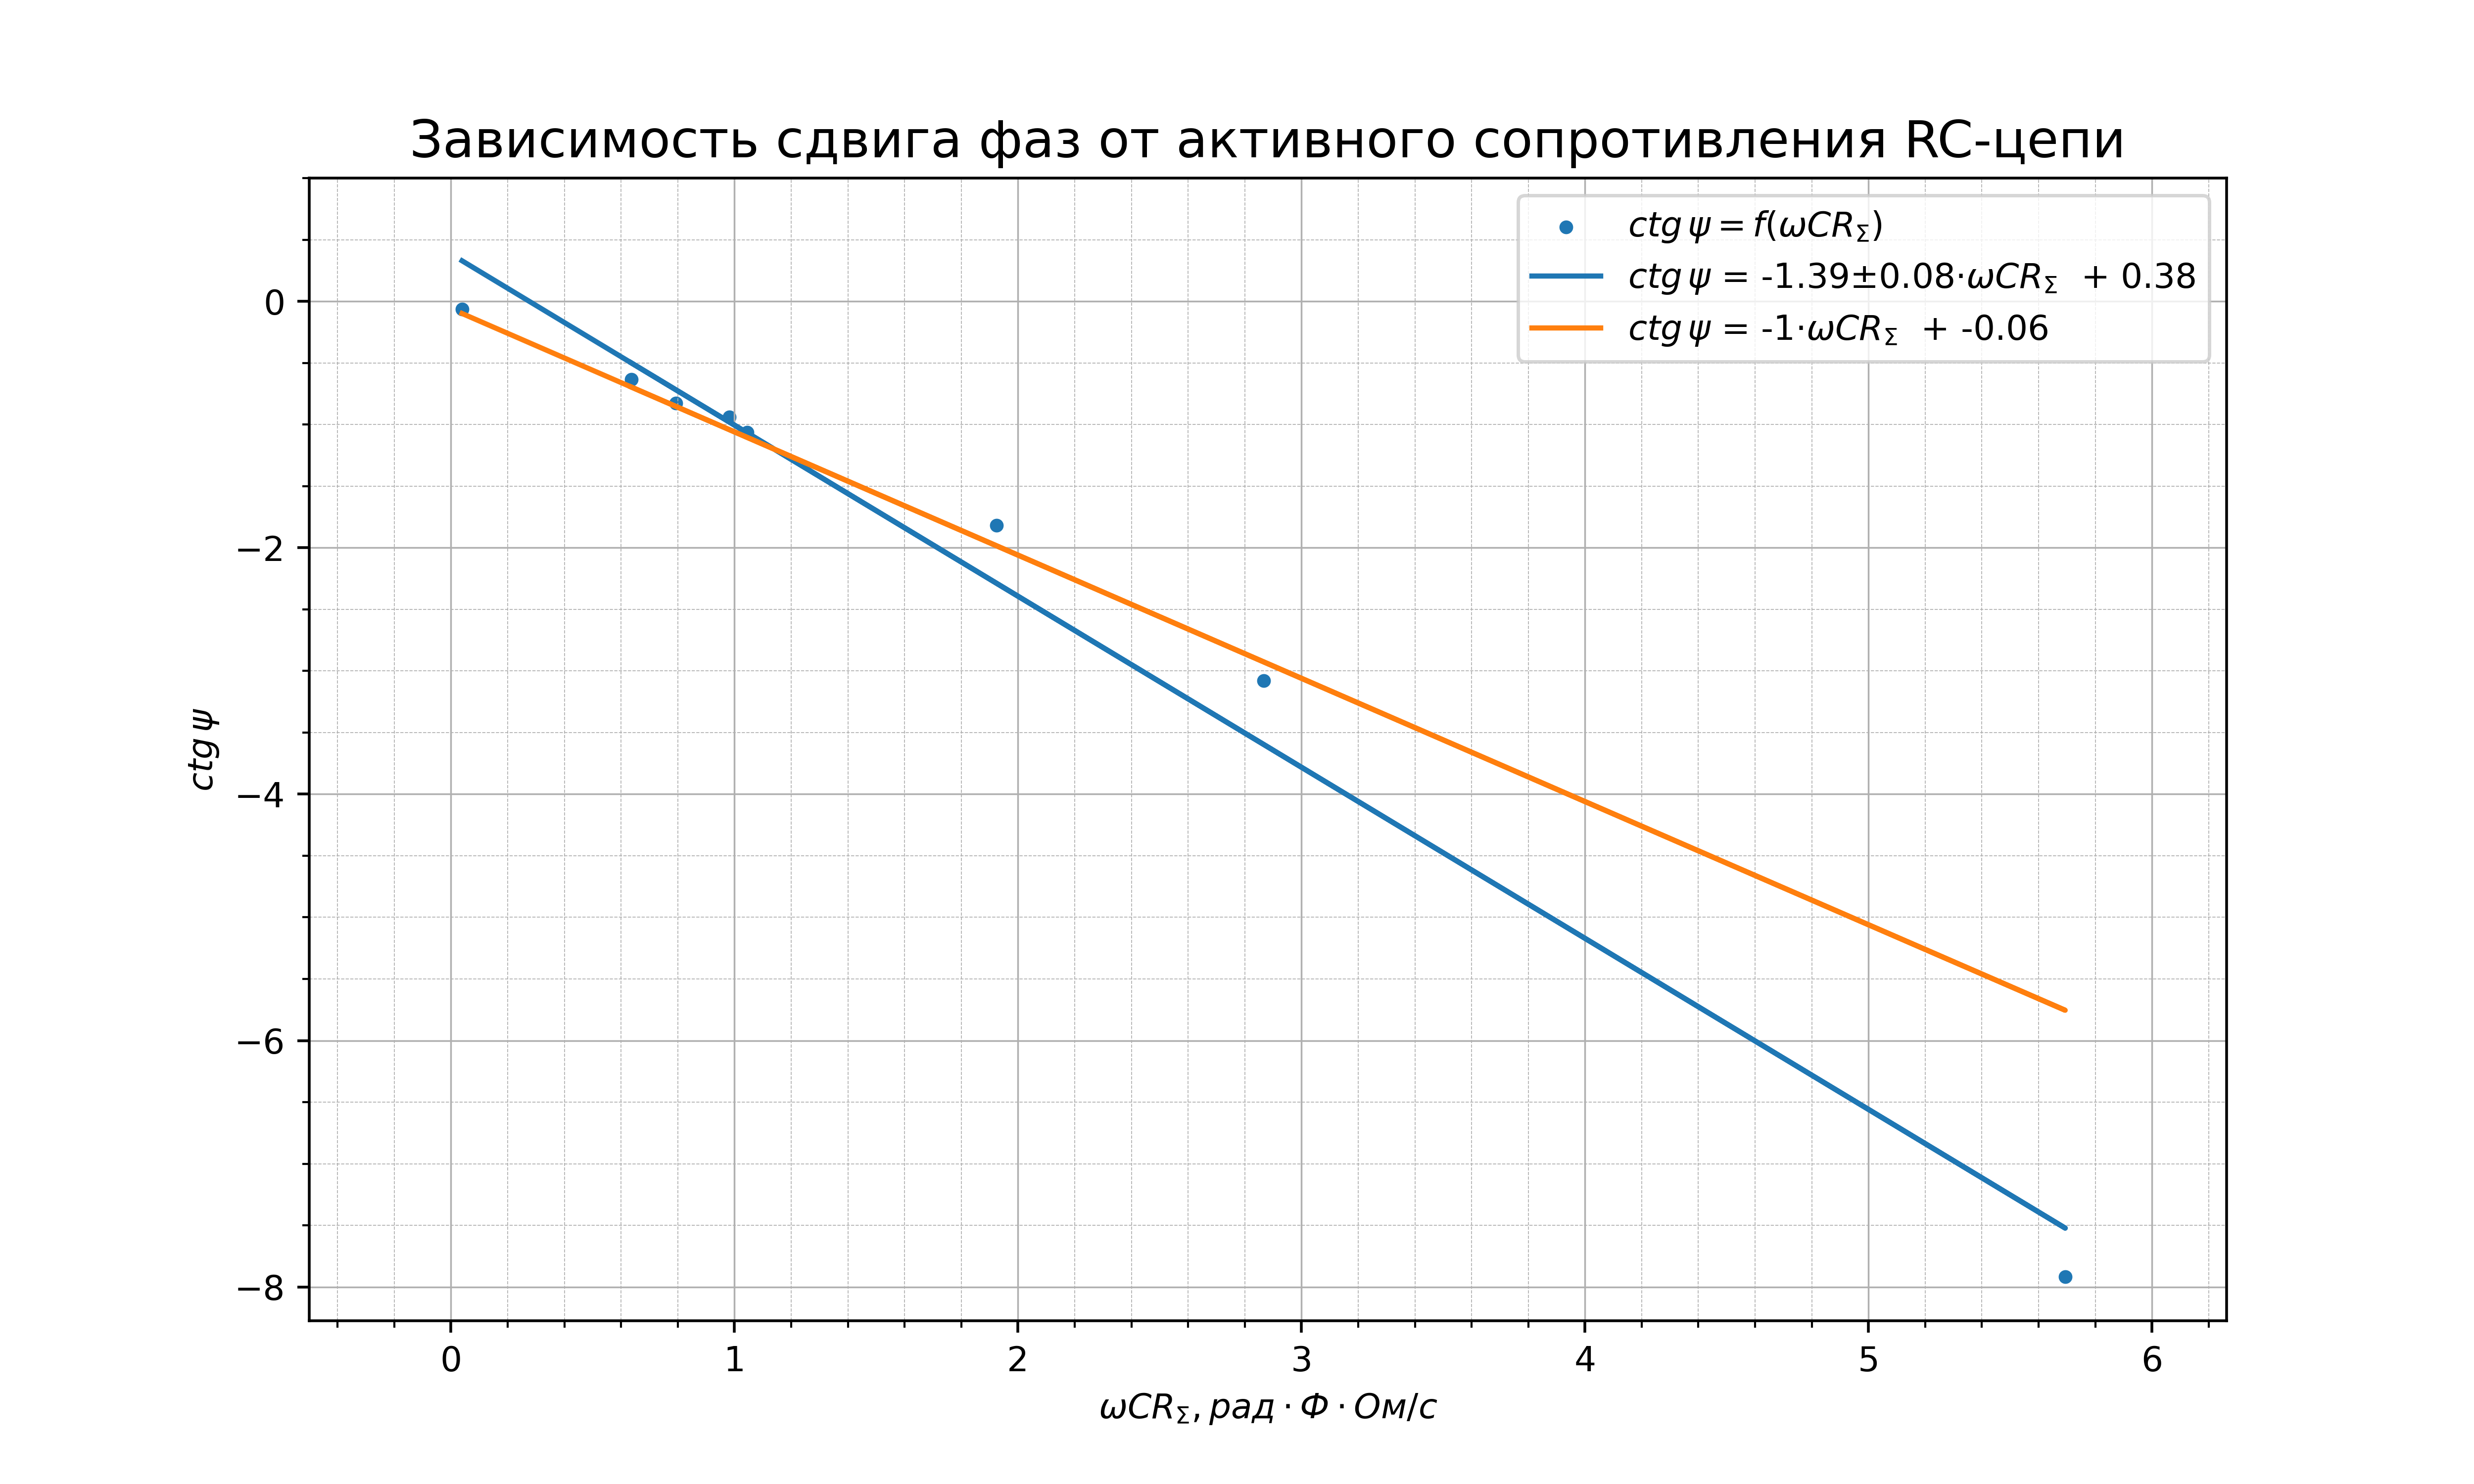
\includegraphics[scale=0.7]{3.2.1_1.png}
\end{flushleft}
\caption{}
\label{ris1}
\end{figure}

\subsection{RL-цепь}

Установленные параметры: $L = 50~мГн,\; \nu = 1~кГц$. Рассчитанное реактивное сопротивление цепи $X_2 = \omega L = 314~Ом$. Полученные значения сдвига фаз $\psi$ в зависимости от сопротивления $R$ представленны в таблице \ref{tab2}.

\begin{table}[h!]
\begin{center}
\begin{tabular}{|c|c|c|c|c|c|c|c|}
\hline
$R, Ом$   & $\sigma_R, Ом$ & $x_0, дел$ & $\sigma_{x_0}, дел$ & $x, дел$ & $\sigma_x, дел$ & $\psi, \pi \cdot рад$ & $\sigma_{\psi}, \pi \cdot рад$ \\ \hline
0,00    & 0,01   & 25,0    & 0,5      & 11,0   & 0,5     & 0,44        & 0,02         \\ \hline
150,00  & 0,01   & 25,0    & 0,5      & 8,0    & 0,5     & 0,32        & 0,02         \\ \hline
380,00  & 0,01   & 25,0    & 0,5      & 5,0    & 0,5     & 0,20        & 0,02         \\ \hline
1110,00 & 0,01   & 25,0    & 0,5      & 2,0    & 0,5     & 0,08        & 0,02         \\ \hline
2110,00 & 0,01   & 25,0    & 0,5      & 1,0    & 0,5     & 0,04        & 0,02         \\ \hline
700,00  & 0,01   & 25,0    & 0,5      & 3,0    & 0,5     & 0,12        & 0,02         \\ \hline
200,00  & 0,01   & 25,0    & 0,5      & 7,0    & 0,5     & 0,28        & 0,02         \\ \hline
50,00   & 0,01   & 25,0    & 0,5      & 10,0   & 0,5     & 0,40        & 0,02         \\ \hline
\end{tabular}
\end{center}
\caption{RL-цепь}
\label{tab2}
\end{table}

Полученный график зависимости $ctg\,\psi = f(R_{\Sigma}/\omega L)$ представлен на рис.~\ref{ris2}. Синим цветом нарисована экспериментальная зависимость, оранжевым --- теоретическая --- $ctg\,\psi~=~R_{\Sigma}/\omega L$. Погрешность экспериментально полученного коэффициента зависимости составляет $\sigma_{RL}~=~14~\%$, что является не очень существенной погрешностью.

\begin{figure}[h!]
\begin{flushleft}
    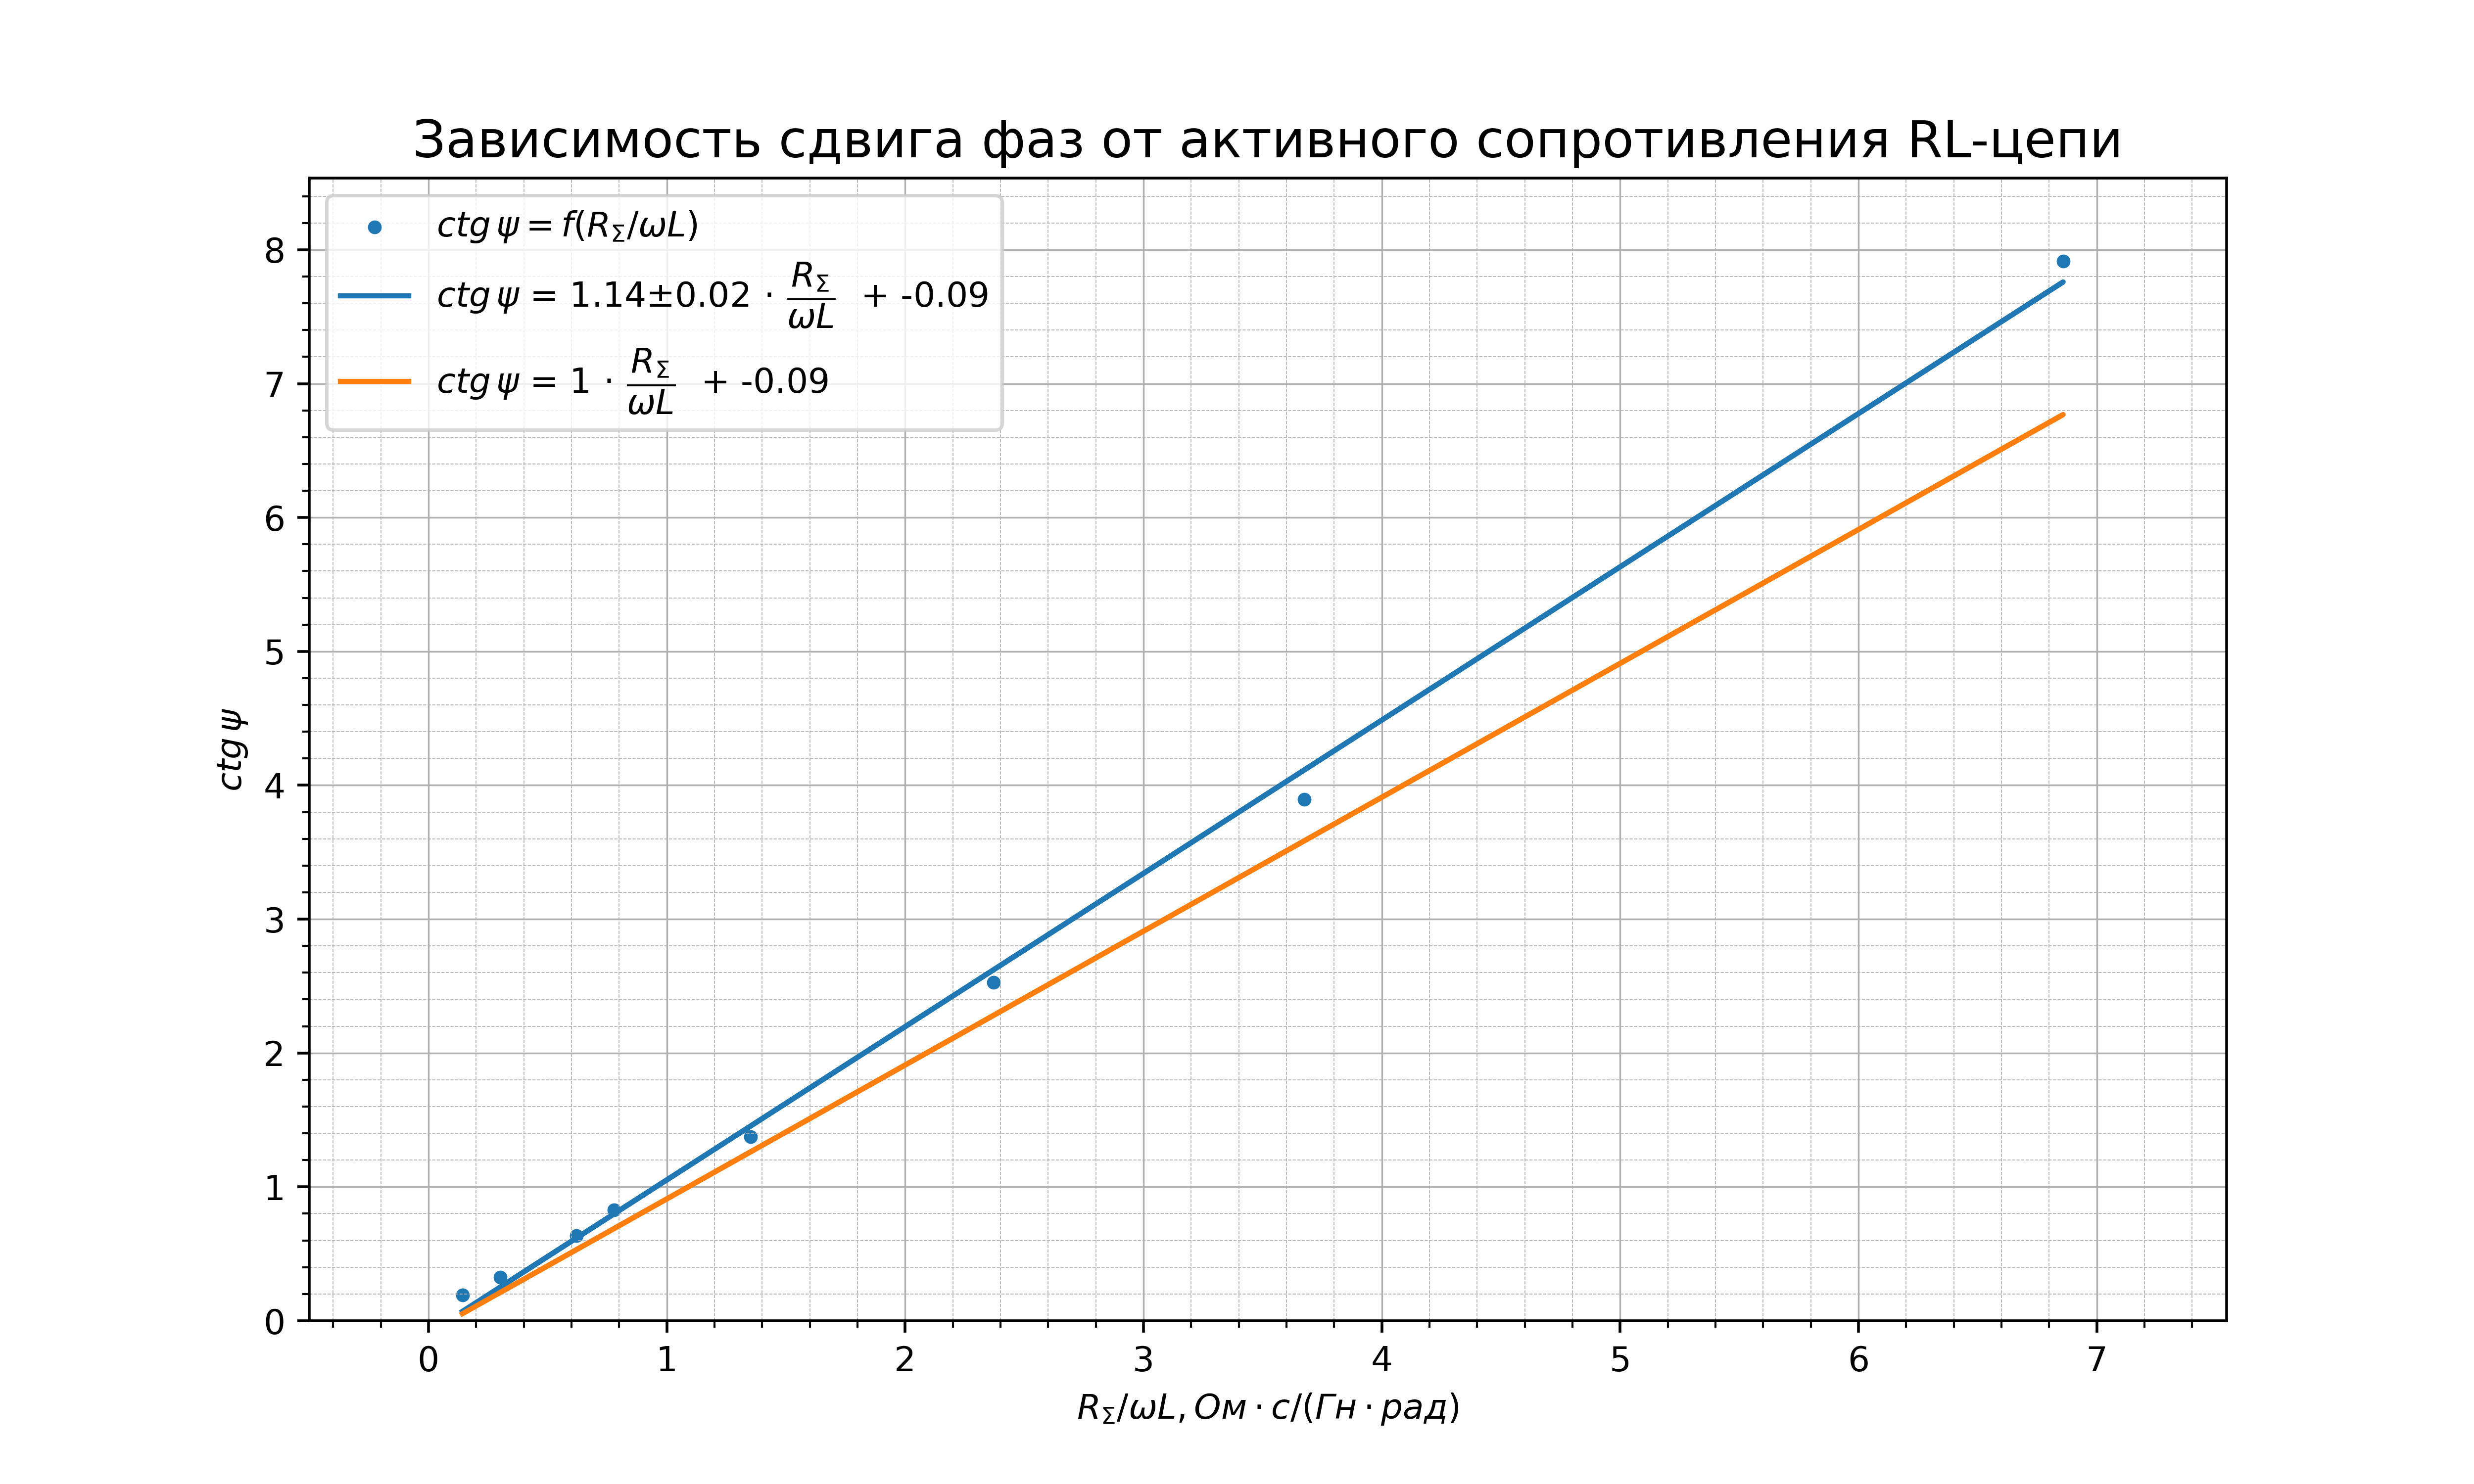
\includegraphics[scale=0.7]{3.2.1_2.png}
\end{flushleft}
\caption{}
\label{ris2}
\end{figure}

\subsection{RLC-цепь}

Установленные параметры: $R = 0,00; 100,00\pm0,01~Ом,\; L = 50,0\pm0,5~мГн, \\ C~=~0,50~\pm~0,01~мкФ$. Рассчитанная резонансная частота цепи $$\nu_0 = 1/(2\pi\sqrt{LC}) = 1007\pm14~Гц.$$ Полученные значения сдвига фаз $\psi$ в зависимости от частоты $\nu$ представленны в таблицах~\ref{tab3}~и~\ref{tab4}.

\begin{table}[h!]
\begin{center}
\begin{tabular}{|c|c|c|c|c|c|c|c|}
\hline
$\nu, Гц$ & $\sigma_{\nu}, Гц$ & $x_0, дел$ & $\sigma_{x_0}, дел$ & $x, дел$ & $\sigma_x, дел$ & $\psi, \pi \cdot рад$ & $\sigma_{\psi}, \pi \cdot рад$ \\ \hline
1000 & 5  & 25,0 & 0,5 & 0,0  & 0,5 & 0,00  & 0,00  \\ \hline 
950  & 5  & 13,0 & 0,5 & -3,0 & 0,5 & -0,2  & 0,04 \\ \hline 
900  & 5  & 14,0 & 0,5 & -4,5 & 0,5 & -0,32 & 0,04 \\ \hline 
920  & 5  & 13,5 & 0,5 & -4,0 & 0,5 & -0,30 & 0,04 \\ \hline 
980  & 5  & 13,0 & 0,5 & -1,0 & 0,5 & -0,08 & 0,04 \\ \hline
970  & 5  & 13,0 & 0,5 & -1,5 & 0,5 & -0,12 & 0,04 \\ \hline
1100 & 10 & 23,0 & 0,5 & 6,0  & 0,5 & 0,26  & 0,02  \\ \hline
1060 & 10 & 24,0 & 0,5 & 4,5  & 0,5 & 0,19  & 0,02  \\ \hline
1140 & 10 & 22,0 & 0,5 & 7,0  & 0,5 & 0,32  & 0,02  \\ \hline
1020 & 10 & 25,0 & 0,5 & 2,0  & 0,5 & 0,08  & 0,02  \\ \hline
1040 & 10 & 24,0 & 0,5 & 3,0  & 0,5 & 0,13  & 0,02  \\ \hline
\end{tabular}
\end{center}
\caption{$R = 0~Ом$}
\label{tab3}
\end{table}

\begin{table}[h!]
\begin{center}
\begin{tabular}{|c|c|c|c|c|c|c|c|}
\hline
$\nu, Гц$ & $\sigma_{\nu}, Гц$ & $x_0, дел$ & $\sigma_{x_0}, дел$ & $x, дел$ & $\sigma_x, дел$ & $\psi, \pi \cdot рад$ & $\sigma_{\psi}, \pi \cdot рад$ \\ \hline
1000 & 5  & 25,0 & 0,5 & 0,0  & 0,5 & 0,00  & 0,00  \\ \hline
980  & 5  & 13,0 & 0,5 & -1,0 & 0,5 & -0,08 & 0,04 \\ \hline
970  & 5  & 13,0 & 0,5 & -1,5 & 0,5 & -0,12 & 0,04 \\ \hline
950  & 5  & 13,0 & 0,5 & -2,0 & 0,5 & -0,15 & 0,04 \\ \hline
920  & 5  & 14,0 & 0,5 & -3,0 & 0,5 & -0,21 & 0,04 \\ \hline
900  & 5  & 14,0 & 0,5 & -3,5 & 0,5 & -0,25 & 0,04 \\ \hline
1020 & 10 & 25,0 & 0,5 & 1,5  & 0,5 & 0,06  & 0,02  \\ \hline
1040 & 10 & 24,0 & 0,5 & 2,5  & 0,5 & 0,10  & 0,02  \\ \hline
1060 & 10 & 24,0 & 0,5 & 3,5  & 0,5 & 0,15  & 0,02  \\ \hline
1100 & 10 & 23,0 & 0,5 & 5,5  & 0,5 & 0,24  & 0,02  \\ \hline
1140 & 10 & 22,0 & 0,5 & 6,5  & 0,5 & 0,30  & 0,02  \\ \hline
\end{tabular}
\end{center}
\caption{$R = 100~Ом$}
\label{tab4}
\end{table}

Полученный график зависимости $|\psi| = f(\nu/\nu_0)$ при $R = 0~Ом$ и $R = 100~Ом$ представлен на рис.~\ref{ris3}. Добротность контура определяется по формуле $$Q = \nu_0/(2\Delta\nu),$$ где $2\Delta\nu$ --- ширина графика при сдвиге фаз $\psi = \pi/4$. Также, добротность можно рассчитать через параметры контура $R_{\Sigma}$, $C$ и $L$: $$Q = \frac{1}{R_{\Sigma}}\sqrt{\frac{L}{C}}.$$ Полученные значения добротности:
\begin{itemize}
\item $R = 0~Ом$: $Q = 6,7\pm0,2$, $Q_{теор} = 7,1\pm0,6$;
\item $R = 100~Ом$: $Q = 2,4\pm0,2$, $Q_{теор} = 2,2\pm0,2$.
\end{itemize}
Полученные значения добротности совпадают с теоретическими в пределах погрешности.

\begin{figure}[h!]
\begin{flushleft}
    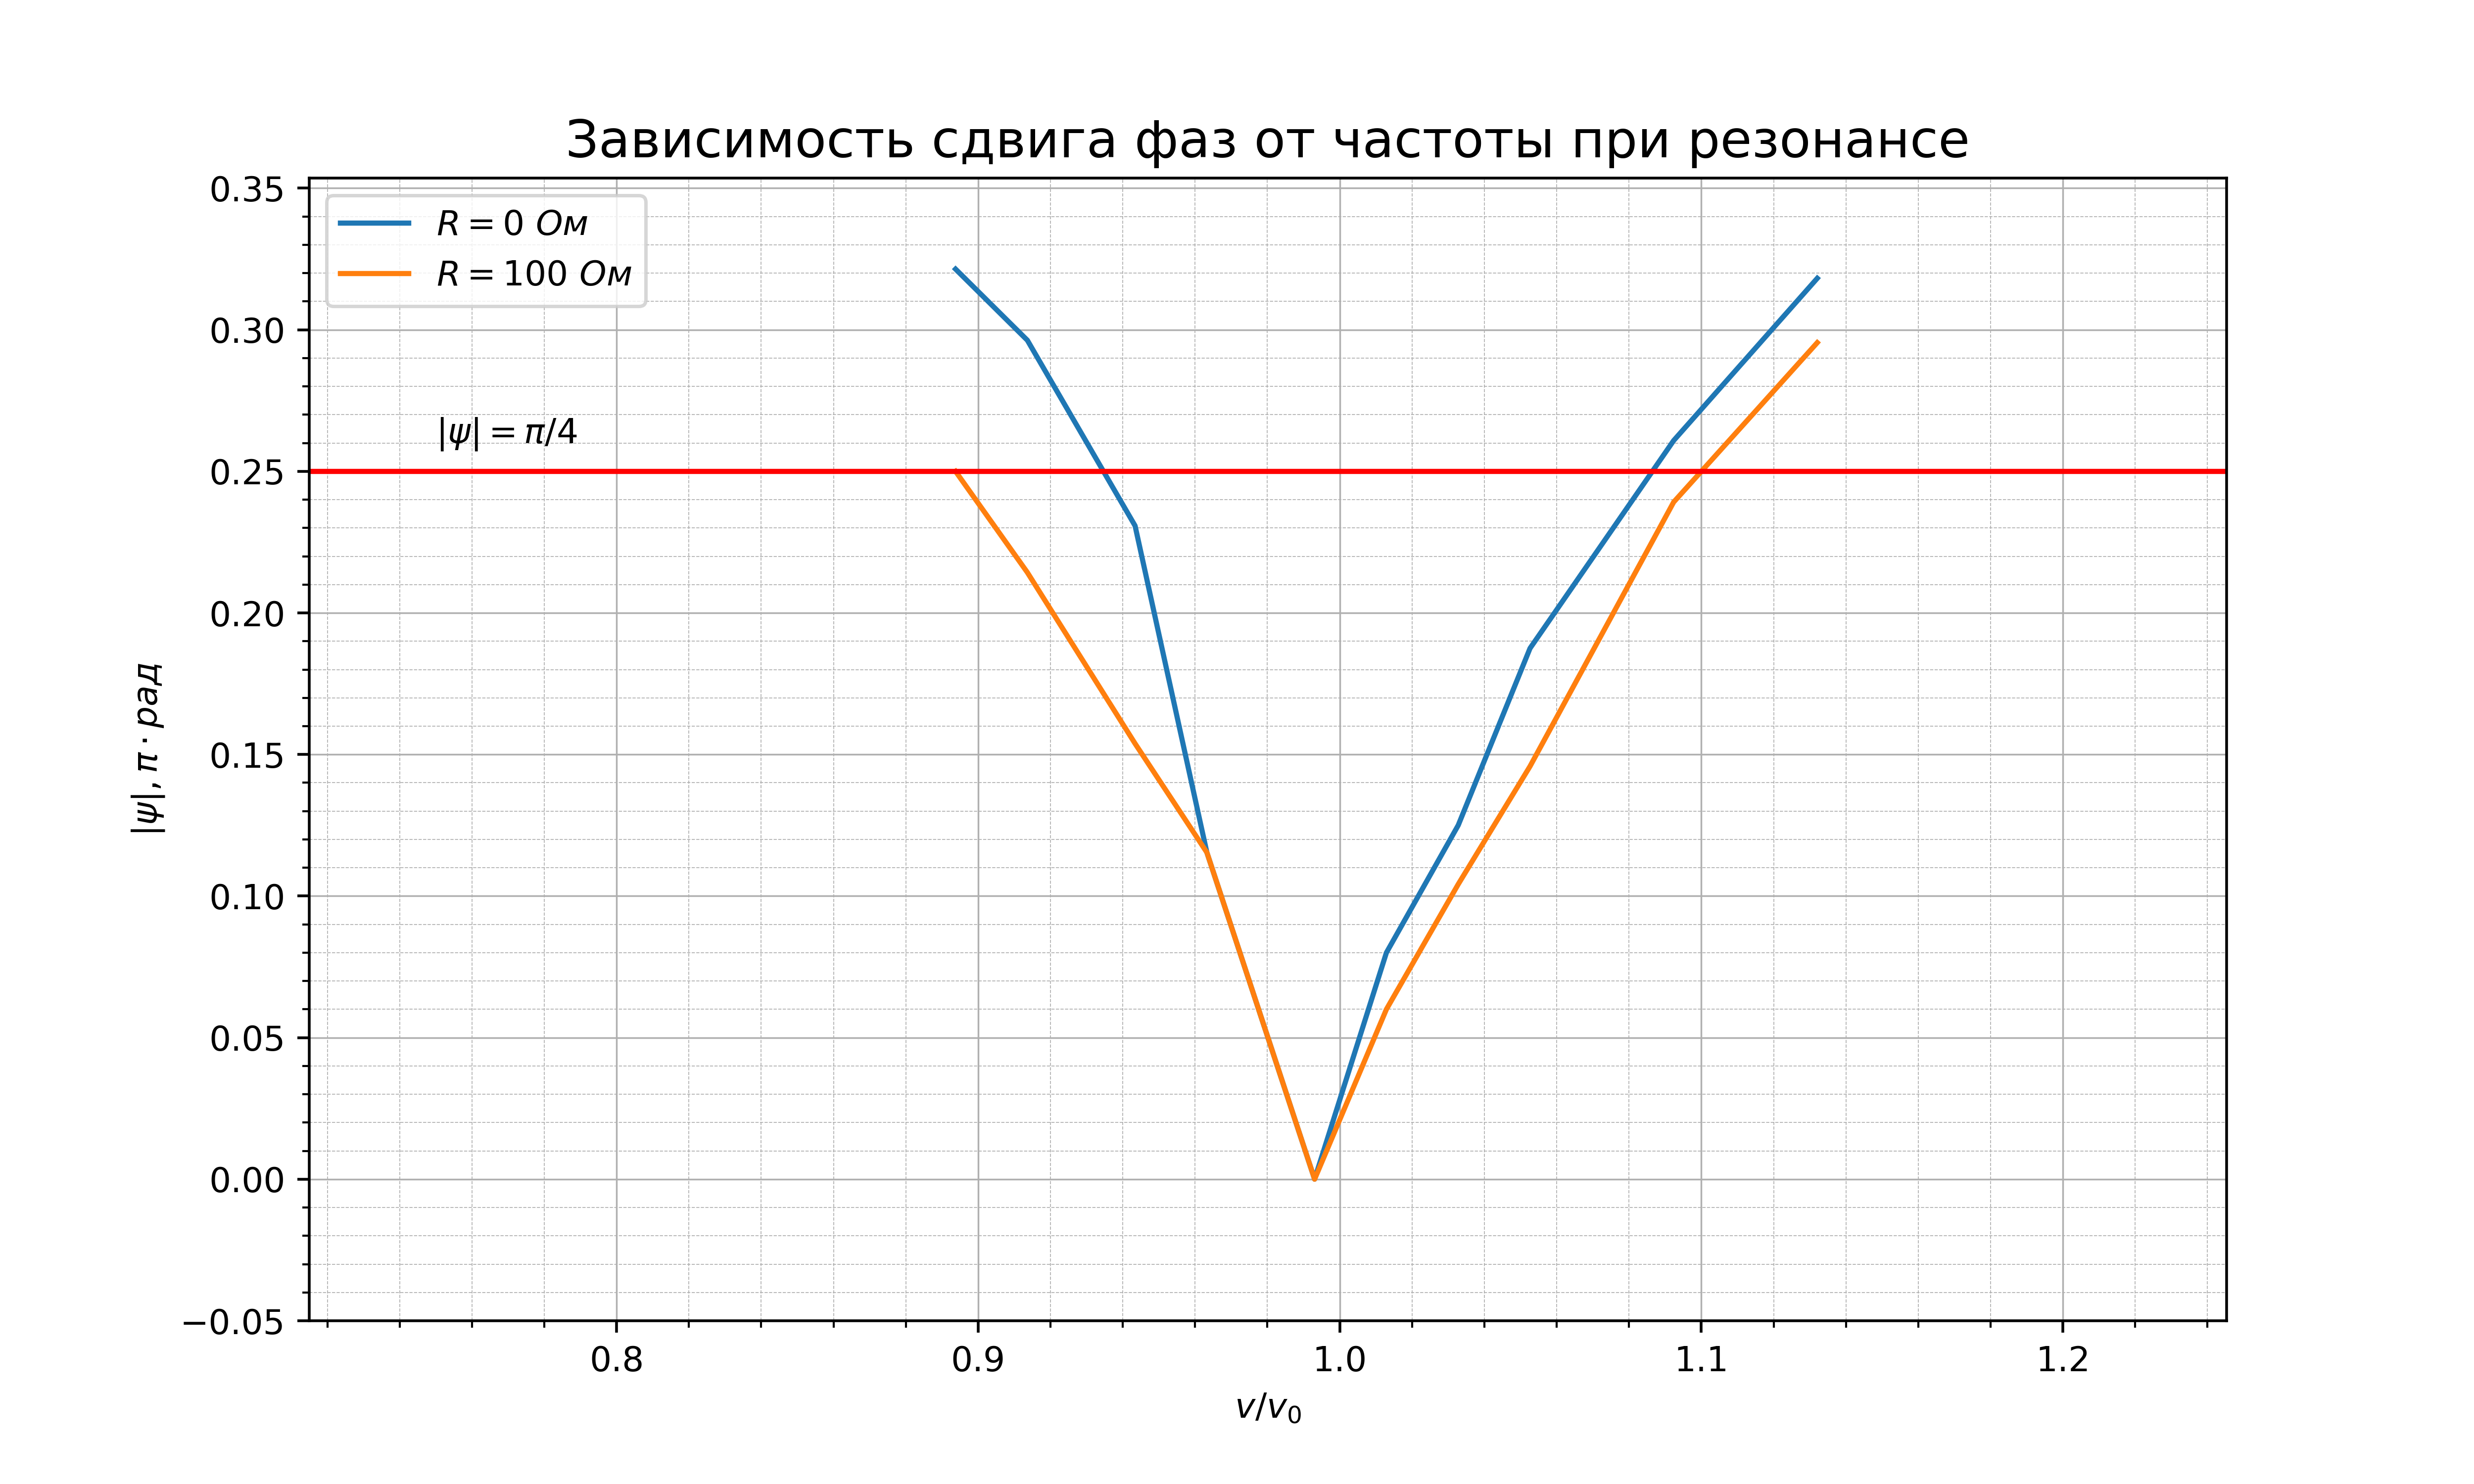
\includegraphics[scale=0.7]{3.2.1_3.png}
\end{flushleft}
\caption{}
\label{ris3}
\end{figure}

\subsection{Фазовращатель}

\begin{figure}[h!]
\begin{center}
    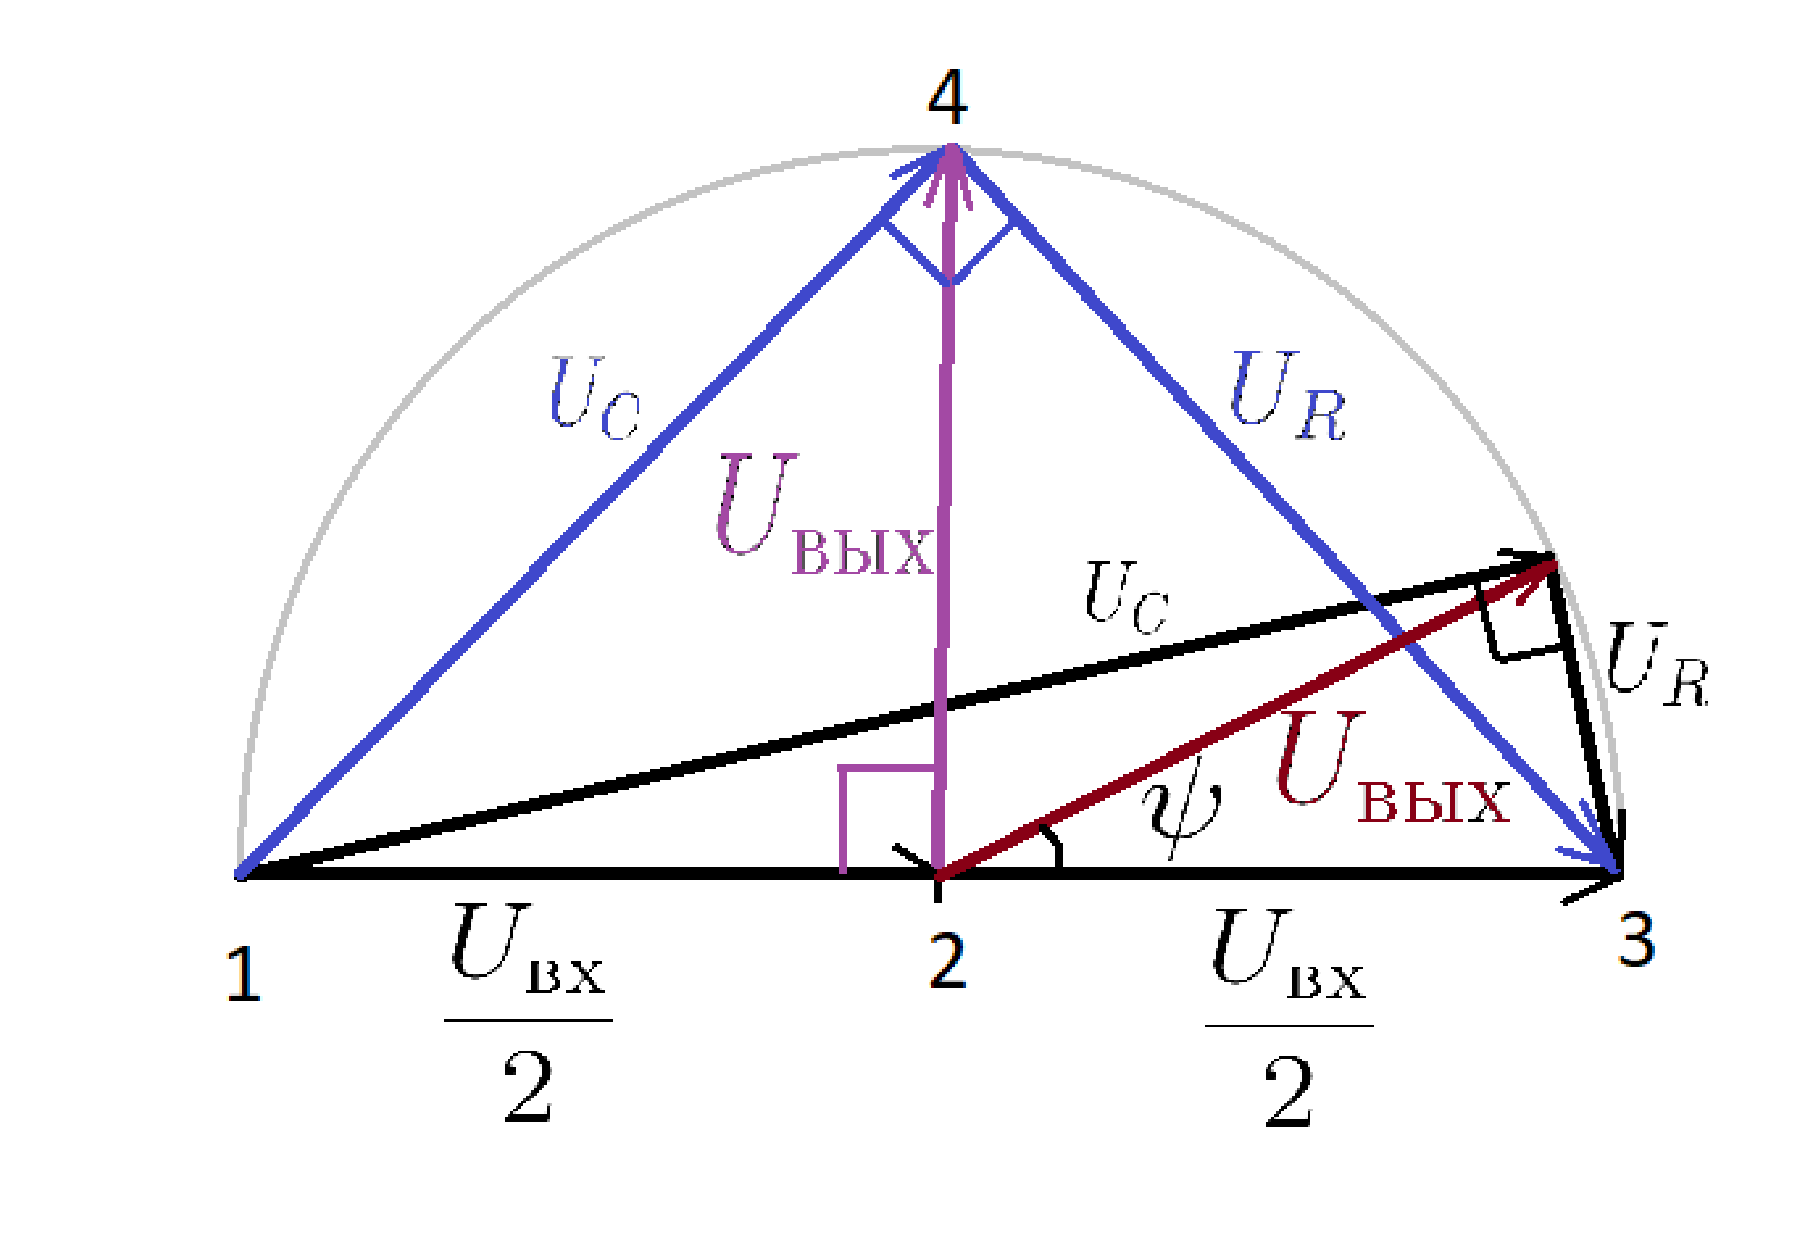
\includegraphics[scale=1.5]{3.2.1_4.png}
\end{center}
\caption{Векторная диаграмма для фазовращателя}
\label{ris4}
\end{figure}

Векторная диаграмма для фазовращателя представлена на рис.~\ref{ris4}. На ней видно, что сдвиг фаз между входным и выходным напряжениями равен $\pi/2$, когда $$\tan{\frac{\psi}{2}} = \tan{\frac{\pi}{4}} = \frac{1}{\omega CR} = 1 \Rightarrow R = \frac{1}{\omega C} = 318~Ом.$$ Экспериментально получено значение $R = 380~Ом$, что существенно отличается от теоретического значения.


Также в данной работе с помощью лабораторного LCR-метра было измерено сопротивление резистора $r$, а также индуктивность $L$ и сопротивление катушки $R_L$. Полученные значения согласуются с указанными на установке:
\begin{itemize}
\item $r = 12,411\pm0,001~Ом$;
\item $R_L = 32,416\pm0,001~Ом$;
\item $L = 50,187\pm0,001~Ом$.
\end{itemize}

\section{Обсуждение результатов и выводы}

В данной работе исследовалась зависимость сдвига фаз в цепи переменного тока от его активного сопротивления при различных параметрах контура. По результатам измерений для RC-цепи зависимость существенно отличается от теоретической, а для RL-цепи согласуется с теорией. Это может быть вызвано плохим контактом соединительных проводов, небольшим количеством измерений или особенностями оборудования в экспериментальной установке.

Добротность исследованной RCL-цепи не превысила 10 при нулевом сопротивлении магазина, а при подключении дополнительного сопротивления и вовсе близка к единице. Это позволяет сделать вывод о том, что данная установка мало подходит для изучения собственных слабозатухающих колебаний в RCL-цепи, так как затухание колебаний в такой цепи будет слишком быстрым. Однако проведённый опыт показал, что полученные значения добротности достаточны для применимости использованной установки при исследовании вынужденных колебаний.

При исследовании фазовращателя рассчитанное теоретически сопротивление магазина, при котором сдвиг фаз между входным и выходным напряжениями равен $\pi/2$, существенно отличается от полученного экспериментально, что может быть вызвано плохим контактом соединительных проводов или особенностями оборудования в экспериментальной установке.

\end{document}